%%%%%%%%%%%%%%%%%%%%%%%%%%%%%%%%%%%%%%%%%
% Funder briefing — Backtest of ICES Advice
% Official Imperial College London Beamer theme
% Compile with XeLaTeX from this directory:
%   xelatex funder_briefing.tex
%%%%%%%%%%%%%%%%%%%%%%%%%%%%%%%%%%%%%%%%%

\documentclass[
  aspectratio=169,
  t,
  onlytextwidth,
  10pt,
]{beamer}

\usetheme{Imperial}

\usepackage{booktabs}
\usepackage{array}
\usepackage{amsmath,amssymb}
\usepackage{colortbl}

\newcommand{\Fmsy}{F_{\mathrm{MSY}}}
\newcommand{\Blim}{B_{\lim}}
\newcommand{\Btrig}{MSYB_{\mathrm{trigger}}}

\title{Backtest of ICES Advice}
\subtitle{Irish Sea whiting and Celtic Sea cod}
\author{Laurence Kell}
\institute{Sea++}
\date{24 August 2026}

\begin{document}

%------------------------------------------------------------------------------
% Title
%------------------------------------------------------------------------------
\begingroup
  \setbeamercolor{background canvas}{bg=ICLBlue}
  \setbeamercolor{title page title}{fg=white}
  \setbeamercolor{title page subtitle}{fg=white}
  \setbeamercolor{author}{fg=white}
  \setbeamercolor{inst}{fg=white}
  \setbeamercolor{date}{fg=white}
  \setbeamertemplate{title page}[logo]{ICL_Logo_White.pdf}
  \frame[plain, s]{\titlepage}
\endgroup

%------------------------------------------------------------------------------
% Agenda
%------------------------------------------------------------------------------
\begingroup
  \setbeamercolor{background canvas}{bg=ICLBlue}
  \setbeamercolor{normal text}{fg=white}\usebeamercolor[fg]{normal text}
  \setbeamercolor{page number in head/foot}{fg=white}
  \begin{frame}
    \begin{columns}[T]
      \begin{column}{0.42\linewidth}
        \HUGE\textbf{Agenda}
      \end{column}
      \begin{column}{0.54\linewidth}
        \textbf{01}\tabto{0.125\linewidth} Why a backtest\\
        \textbf{02}\tabto{0.125\linewidth} Case-study stocks\\
        \textbf{03}\tabto{0.125\linewidth} Method\\
        \textbf{04}\tabto{0.125\linewidth} Take-home: two stocks\\
        \textbf{05}\tabto{0.125\linewidth} Remaining questions\\
        \textbf{06}\tabto{0.125\linewidth} Next steps
      \end{column}
    \end{columns}
  \end{frame}
\endgroup

%------------------------------------------------------------------------------
% Why
%------------------------------------------------------------------------------
\begin{frame}
  \frametitle{Two questions that are often mixed}
  \framesubtitle{Why this project}

  \begin{columns}[T]
    \begin{column}{0.48\linewidth}
      \textbf{Was the science robust?}\\[0.4em]
      Given the assessment and harvest control rule in force at the time, would following advice have delivered the intended status, yield and stability?
    \end{column}
    \begin{column}{0.48\linewidth}
      \textbf{Was advice followed?}\\[0.4em]
      Did realised catch match advised catch? If not, how much of the poor outcome is implementation, not the rule itself?
    \end{column}
  \end{columns}

  \vspace{0.8em}
  A \textbf{backtest} is a retrospective management strategy evaluation:
  reconstruct each year's perception, apply that year's rule, project under
  perfect implementation, and compare with what actually happened.
\end{frame}

\begin{frame}
  \frametitle{What success looks like}
  \framesubtitle{For management, not only for the model}

  \begin{itemize}
    \item Separate \textbf{implementation failure} from \textbf{advice-rule failure}.
    \item Show, stock by stock, whether following advice would have rebuilt biomass, reduced overfishing, or mainly changed yield in the short term.
    \item Identify where the ICES MSY rule itself is the constraint (zero-catch advice, unstable assessments, benchmark breaks).
    \item Leave a reproducible workflow that can be updated as new assessments arrive.
  \end{itemize}
\end{frame}

%------------------------------------------------------------------------------
% Stocks
%------------------------------------------------------------------------------
\begin{frame}
  \frametitle{Six Category~1 case studies}
  \framesubtitle{All retained after week-1 screening}

  {\small
  \begin{tabular}{@{}llll@{}}
    \toprule
    Stock & Area & Assessment & Advice basis \\
    \midrule
    Irish Sea cod & 7.a & Age-structured & ICES MSY \\
    Irish Sea whiting & 7.a & SAM & ICES MSY \\
    Celtic Sea cod & 7.e--k & SAM & ICES MSY \\
    Celtic Sea whiting & 7.b--c, 7.e--k & Age-based & ICES MSY \\
    Celtic Sea haddock & 7.b--k & SAM & ICES MSY \\
    NE Atlantic mackerel & 1--8, 14, 9.a & Integrated & Coastal States MSY \\
    \bottomrule
  \end{tabular}}

  \vspace{0.6em}
  SAG coverage is typically 2016/17--2025/26 (about 8--10 assessment years).
  Irish Sea whiting is the sparsest; mackerel is retained \textbf{provisionally}.
\end{frame}

%------------------------------------------------------------------------------
% Method + progress
%------------------------------------------------------------------------------
\begin{frame}
  \frametitle{How the backtest works}
  \framesubtitle{Repeated for each historical assessment year $t$}

  \begin{enumerate}
    \item \textbf{Perception} --- reconstruct status using only data and reference points available at $t$.
    \item \textbf{Advice} --- apply the harvest control rule then in force
          ($F=\Fmsy$ above $\Btrig$; linear reduction to zero at $\Blim$).
    \item \textbf{Counterfactual} --- project the operating model with catch equal to advised catch (perfect implementation).
    \item \textbf{Compare} --- SSB, $F$, catch, time below $\Blim$/$\Btrig$, versus realised history.
  \end{enumerate}
\end{frame}

\begin{frame}
  \frametitle{Where we are}
  \framesubtitle{Contract workplan: 50 days}

  {\small
  \begin{tabular}{@{}lp{0.42\linewidth}ll@{}}
    \toprule
    Task & Content & Days & Status \\
    \midrule
    1 & Screening, status, catch vs advice, open-loop $F$ checks & 5 & \textbf{Done} \\
    2 & Assessment reconstruction (historical peels) & 20 & Prototype \\
    3 & Operating models and perfect-management HCR runs & 15 & \textbf{In progress} \\
    4 & Metrics, synthesis, technical report & 10 & Draft shell \\
    \bottomrule
  \end{tabular}}

  \vspace{0.7em}
  Screening delivered. Operating models and open-loop $F$ projections are run.
  Closed-loop HCR, peels, and Historical / Current / Future remain.
\end{frame}

%------------------------------------------------------------------------------
% Results
%------------------------------------------------------------------------------
\begingroup
  \setbeamercolor{background canvas}{bg=ICLBlue}
  \setbeamercolor{normal text}{fg=white}\usebeamercolor[fg]{normal text}
  \setbeamercolor{page number in head/foot}{fg=white}
  \begin{frame}
    \begin{adjustwidth}{0cm}{0.12\textwidth}
      {\Huge\ImperialSansSemiBold Take-home: two stocks}
    \end{adjustwidth}
  \end{frame}
\endgroup

\begin{frame}
  \frametitle{If advice had been followed}
  \framesubtitle{Same observed productivity; only harvest policy changes}

  {\footnotesize
  \begin{tabular}{@{}p{0.28\linewidth}p{0.33\linewidth}p{0.33\linewidth}@{}}
    \toprule
     & Irish Sea whiting & Celtic Sea cod \\
    \midrule
    Latest status
      & Below $B_{\mathrm{trigger}}$; $F$ is not the whole story
      & Far below $B_{\lim}$; $F\gg F_{\mathrm{target}}$ \\[0.6em]
    $F=F_{\mathrm{target}}$ from 1990
      & SSB rebuilds to several times $B_{\mathrm{trigger}}$
      & Large biomass gain once $F$ is cut \\[0.6em]
    Advice rule from 2015
      & Already above trigger and OM $B_{\mathrm{MSY}}$ at the start
      & Can sit above the trigger and still short of OM $B_{\mathrm{MSY}}$ \\[0.6em]
    What this is not
      & Climate projection. Residuals, $M$, mass and maturity are observed productivity.
      & Same. \\
    \bottomrule
  \end{tabular}}

  \vspace{0.5em}
  {\small Historical / Current replay recruitment residuals.
  Future (20-year rebuild) uses mean recruitment --- a different experiment.}
\end{frame}

\begin{frame}
  \frametitle{Latest status is poor for most stocks}
  \framesubtitle{SAG terminal year relative to current reference points}

  {\footnotesize
  \begin{tabular}{@{}lrrr@{}}
    \toprule
    Stock & SSB/$\Btrig$ & SSB/$\Blim$ & $F/\Fmsy$ \\
    \midrule
    Irish Sea cod        & 0.28 & 0.38 & 0.05 \\
    Irish Sea whiting    & 0.63 & 0.87 & --- \\
    Celtic Sea cod       & 0.02 & 0.02 & 4.95 \\
    Celtic Sea whiting   & 0.26 & 0.36 & 0.65 \\
    Celtic Sea haddock   & 0.63 & 0.88 & 1.78 \\
    NE Atlantic mackerel & 0.77 & 1.03 & 1.39 \\
    \bottomrule
  \end{tabular}}

  \vspace{0.5em}
  \begin{itemize}
    \item All six are below $\Btrig$; Celtic Sea cod is far below $\Blim$.
    \item Celtic Sea cod, haddock and mackerel: $F>\Fmsy$ in the latest year.
    \item Irish Sea cod: $F$ already low, but biomass has not rebuilt --- weak year classes since $\sim$2020.
  \end{itemize}
\end{frame}

\begin{frame}
  \frametitle{Advice was often not followed}
  \framesubtitle{Reported catch versus ICES advised catch}

  \begin{itemize}
    \item \textbf{Celtic and Irish Sea cod and whiting:} advised catch cuts were not fully taken.
    \item \textbf{Mackerel:} catch has consistently exceeded advice.
    \item \textbf{Celtic Sea haddock:} catch has generally been \emph{below} advice --- a different kind of mismatch.
  \end{itemize}

  \vspace{0.4em}
  That gap is why a backtest is informative.
  If advice had always been followed, we could only test the science, not management effectiveness.

  \vspace{0.4em}
  {\small Screening uses catch versus advice only --- not TAC. Perfect-management runs assume catch $=$ advised catch.}
\end{frame}

\IfFileExists{../figs/week1_catch_advice.pdf}{%
\begin{frame}
  \frametitle{Catch versus advised catch}
  \framesubtitle{SAG reported catch vs ASD advice (independent $y$-axes)}
  \includegraphics[width=0.98\textwidth,height=0.72\textheight,keepaspectratio]{../figs/week1_catch_advice.pdf}
\end{frame}}{}

\IfFileExists{../figs/week1_sag_ssb.pdf}{%
\begin{frame}
  \frametitle{SSB perception changes with each assessment}
  \framesubtitle{SAG spawning-stock biomass by assessment year}
  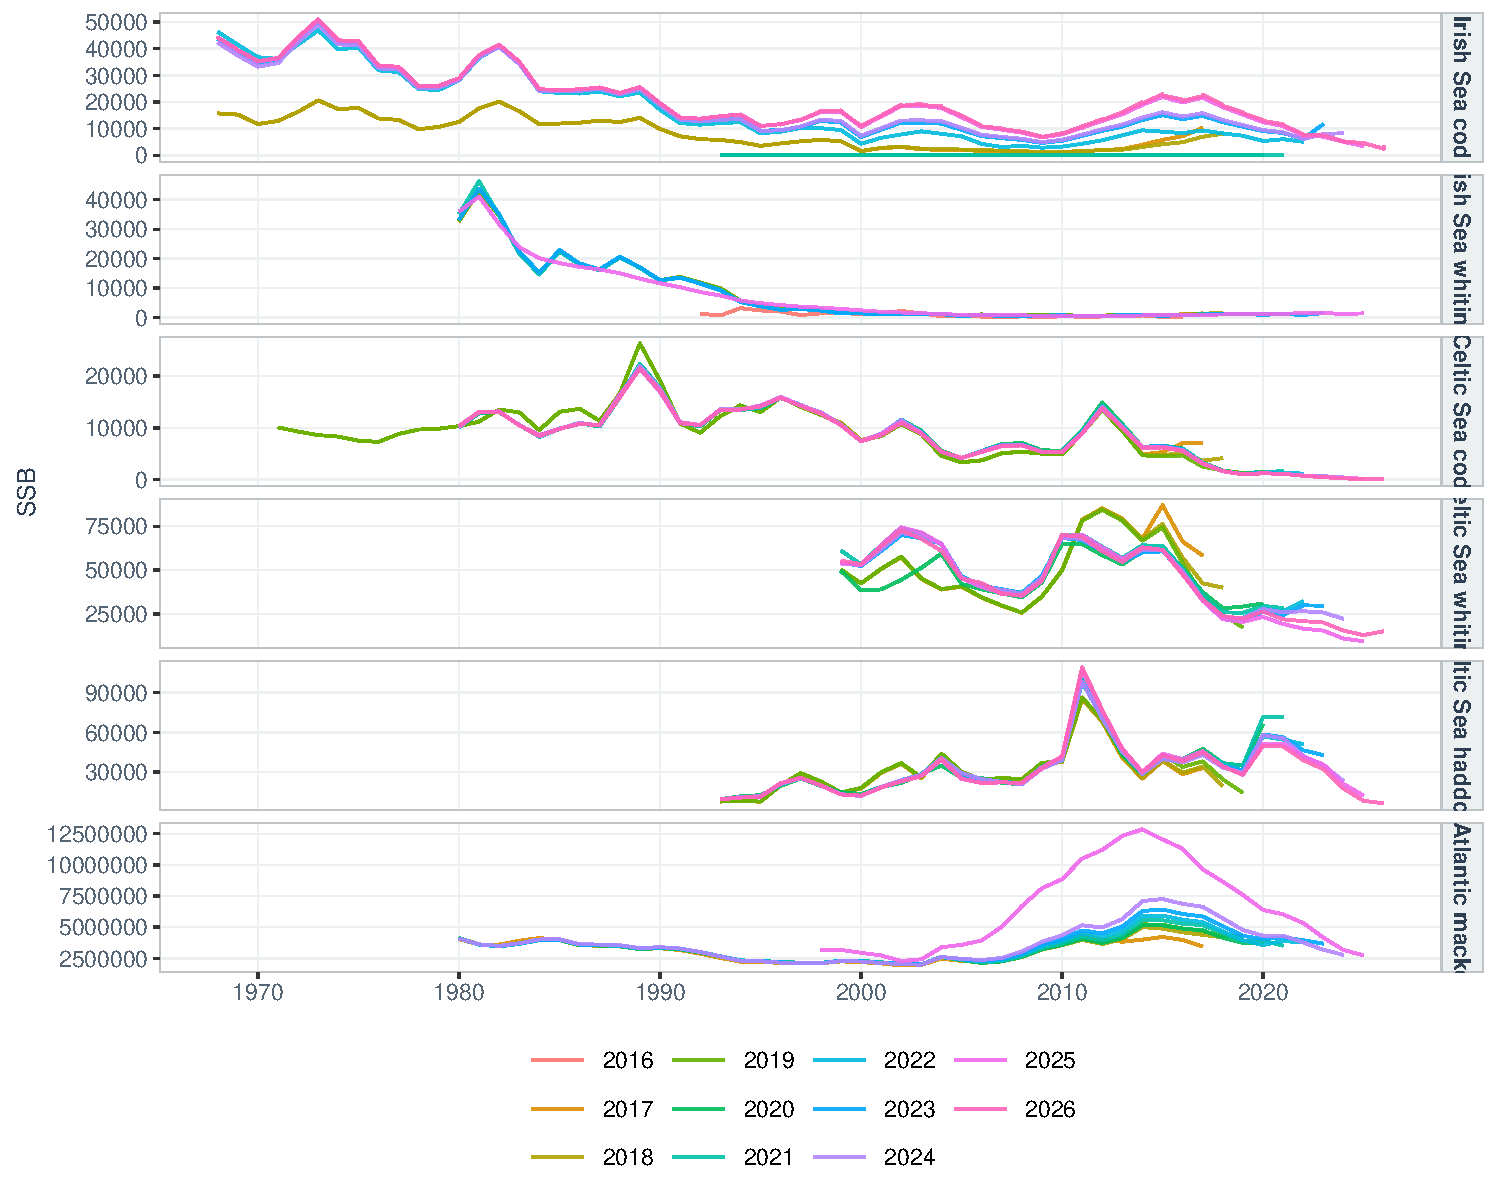
\includegraphics[width=0.98\textwidth,height=0.72\textheight,keepaspectratio]{../figs/week1_sag_ssb.pdf}
\end{frame}}{}

\IfFileExists{../figs/week1_projections.pdf}{%
\begin{frame}
  \frametitle{Open-loop $F_{\mathrm{MSY}}$ projections}
  \framesubtitle{Actual vs mean recruitment vs recruitment deviates}
  \includegraphics[width=0.98\textwidth,height=0.72\textheight,keepaspectratio]{../figs/week1_projections.pdf}
\end{frame}}{}

\begin{frame}
  \frametitle{Constant-$F$ checks: fishing vs recruitment}
  \framesubtitle{Open-loop screening projections, not the closed-loop backtest}

  Three tracks at the same target $F=\Fmsy$:
  \begin{itemize}
    \item \textbf{Actual} --- realised $F$ and recruitment.
    \item \textbf{Mean recruitment} --- isolates a deterministic $F$ effect.
    \item \textbf{Recruitment deviates} --- same $F$, historical year-class pattern.
  \end{itemize}

  \vspace{0.3em}
  \textbf{What this already suggests}
  \begin{itemize}
    \item Celtic Sea cod: $F\gg\Fmsy$, SSB $\ll\Blim$ --- following a lower $F$ is the clearest screening case for higher biomass.
    \item Celtic Sea whiting: biomass poor but $F<\Fmsy$; recruitment, not only $F$, is driving the path.
    \item Irish Sea cod: low $F$ has not rebuilt the stock; the counterfactual is not ``just fish less''.
  \end{itemize}
\end{frame}

\begin{frame}
  \frametitle{Assessments move: updates vs benchmarks}
  \framesubtitle{Perception of status is not a fixed time series}

  \begin{itemize}
    \item Update years mainly revise the most recent points (usual retrospective fan).
    \item Benchmarks can change \textbf{scale and reference points} --- mackerel, Celtic Sea whiting, Irish Sea cod.
    \item For mackerel the recent benchmark shifted both the stock trend and the reference-point basis. Screening numbers for that stock are \textbf{provisional}.
  \end{itemize}

  \vspace{0.5em}
  The backtest must use \textbf{the reference points in force in year $t$}, not only today's $\Fmsy$ and $\Btrig$.
\end{frame}

\begin{frame}
  \frametitle{Screening decision}
  \framesubtitle{What we have already taken as given}

  \begin{itemize}
    \item \textbf{Proceed with all six stocks.} No alternative list proposed.
    \item Mackerel kept, but benchmark handling must be agreed before full conditioning.
    \item Operating-model biology can follow the assessment; the critical choice is the \textbf{stock--recruitment relationship} and how deviates are used in projection.
    \item Short-term reference projections from the \emph{latest} assessment (as in the project plan) are still outstanding --- distinct from the whole-period screening runs.
  \end{itemize}
\end{frame}

%------------------------------------------------------------------------------
% Questions
%------------------------------------------------------------------------------
\begingroup
  \setbeamercolor{background canvas}{bg=ICLBlue}
  \setbeamercolor{normal text}{fg=white}\usebeamercolor[fg]{normal text}
  \setbeamercolor{page number in head/foot}{fg=white}
  \begin{frame}
    \begin{adjustwidth}{0cm}{0.08\textwidth}
      {\Huge\ImperialSansSemiBold Questions where we need clarity}
    \end{adjustwidth}
  \end{frame}
\endgroup

\begin{frame}
  \frametitle{Q1 --- Mackerel}
  \framesubtitle{Retain, special-case, or drop?}

  {\large The recent benchmark changed perceived scale and reference points, not only the last few years.}

  \vspace{0.6em}
  \textbf{What I need from you}
  \begin{itemize}
    \item Keep it as a full sixth case study?
    \item Keep it, but freeze pre-benchmark reference points / scale with an agreed rule?
    \item Park it until the other five are done, then return?
  \end{itemize}

  \vspace{0.4em}
  {\small This is the highest-risk stock in the set. Getting the rule wrong will dominate the narrative.}
\end{frame}

\begin{frame}
  \frametitle{Q2 --- How far back do we peel?}
  \framesubtitle{Assessment window}

  {\large Practical window is about \textbf{8--10 years} (2016/17--2025/26).}

  \vspace{0.6em}
  \textbf{What I need from you}
  \begin{itemize}
    \item Is that long enough for the decision you want to support?
    \item Prefer a common window across stocks, or the maximum SAG years per stock?
    \item Irish Sea whiting has gaps and recent zero-catch advice --- same window, or a shorter documented subset?
  \end{itemize}
\end{frame}

\begin{frame}
  \frametitle{Q3 --- Reconstructing historical assessments}
  \framesubtitle{SAG gives outputs, not the inputs as they stood in year $t$}

  {\large We cannot fully rerun ``the assessment as published'' from SAG archives alone.}

  \vspace{0.6em}
  \textbf{Options}
  \begin{enumerate}
    \item \textbf{Simulation:} hold catch-at-age and biology; simulate CPUE; rerun SAM --- closer to a true peel, more work.
    \item \textbf{Approximate peels} from the latest assessment --- faster, weaker claim.
    \item \textbf{Hybrid:} simulation on one or two stocks; approximation on the rest.
  \end{enumerate}

  \vspace{0.3em}
  Which claim do you need the report to be able to make?
\end{frame}

\begin{frame}
  \frametitle{Q4 --- What does ``perfect management'' mean?}
  \framesubtitle{The counterfactual definition}

  Screening compared \textbf{catch vs advised catch}. TAC is not in the figures yet.

  \vspace{0.5em}
  \textbf{What I need from you}
  \begin{itemize}
    \item Is the policy question ``what if catch had equalled ICES advice''?
    \item Or do we also need TAC vs advice vs catch (three-way mismatch)?
    \item For years with \textbf{zero-catch advice} (Irish Sea whiting), is the intended story ``perfect management means no fishing'', even if that makes short-term yield look worse by design?
  \end{itemize}
\end{frame}

\begin{frame}
  \frametitle{Q5 --- What decision should the report serve?}
  \framesubtitle{This shapes metrics, depth, and how we spend the remaining days}

  Possible uses (not mutually exclusive):
  \begin{itemize}
    \item Show managers the cost of not following advice.
    \item Test whether the ICES MSY rule would have rebuilt these stocks if followed.
    \item Inform HCR / long-term management plan discussions (including rebuilding).
    \item A technical methods report, with policy implications secondary.
  \end{itemize}

  \vspace{0.4em}
  {\large Which of these is primary for you?}
\end{frame}

\begin{frame}
  \frametitle{Q6 --- Sequencing and depth}
  \framesubtitle{About 45 days remain}

  \textbf{Proposal:} one stock end-to-end first (Celtic Sea cod is the clearest screening case), then roll the same workflow across the others.

  \vspace{0.5em}
  \textbf{What I need from you}
  \begin{itemize}
    \item Agree Celtic Sea cod as the prototype, or nominate another?
    \item Equal depth on all six, or a full treatment plus lighter companions?
    \item Final package: technical report only, or also a short briefing note / these slides updated with counterfactuals?
  \end{itemize}
\end{frame}

\begin{frame}
  \frametitle{What I need from this meeting}
  \framesubtitle{A usable decision on each}

  {\small
  \begin{tabular}{@{}lp{0.72\linewidth}@{}}
    \toprule
    & Decision \\
    \midrule
    Q1 & Mackerel: full case / special rule / defer \\
    Q2 & Peel window: common years vs maximum per stock \\
    Q3 & Reconstruction: simulation, approximation, or hybrid \\
    Q4 & Counterfactual: catch $=$ advice; TAC or not; zero-catch years \\
    Q5 & Primary use of the report \\
    Q6 & Prototype stock and depth vs breadth \\
    \bottomrule
  \end{tabular}}
\end{frame}

%------------------------------------------------------------------------------
% Next / close
%------------------------------------------------------------------------------
\begin{frame}
  \frametitle{Immediate next steps (after today)}

  \begin{enumerate}
    \item Funder HTML note: \texttt{Rmd/06.1\_TwoStocks.html}
          (Irish Sea whiting, Celtic Sea cod).
    \item All-stock digest (\texttt{05.0}) then the next case study.
    \item SAM observation error (\texttt{04.4}) as robustness, not the base case.
    \item Draft ICESJMS outline in \texttt{docs/paper\_outline.md}.
  \end{enumerate}

  \vspace{0.5em}
  Screening PDF and the gated OM remain contract deliverables.
\end{frame}

\begingroup
  \setbeamercolor{background canvas}{bg=ICLBlue}
  \setbeamercolor{normal text}{fg=white}\usebeamercolor[fg]{normal text}
  \setbeamercolor{title page title}{fg=white}
  \setbeamercolor{date}{fg=white}
  \setbeamertemplate{closing slide logo}[logo]{ICL_Logo_White.pdf}
  \setbeamertemplate{closing slide text}[text]{Happy to discuss}
  \usebeamertemplate{closing slide}
\endgroup

\end{document}
